% Options for packages loaded elsewhere
\PassOptionsToPackage{unicode}{hyperref}
\PassOptionsToPackage{hyphens}{url}
\PassOptionsToPackage{dvipsnames,svgnames,x11names}{xcolor}
%
\documentclass[
]{article}
\usepackage{amsmath,amssymb}
\usepackage{iftex}
\ifPDFTeX
  \usepackage[T1]{fontenc}
  \usepackage[utf8]{inputenc}
  \usepackage{textcomp} % provide euro and other symbols
\else % if luatex or xetex
  \usepackage{unicode-math} % this also loads fontspec
  \defaultfontfeatures{Scale=MatchLowercase}
  \defaultfontfeatures[\rmfamily]{Ligatures=TeX,Scale=1}
\fi
\usepackage{lmodern}
\ifPDFTeX\else
  % xetex/luatex font selection
\fi
% Use upquote if available, for straight quotes in verbatim environments
\IfFileExists{upquote.sty}{\usepackage{upquote}}{}
\IfFileExists{microtype.sty}{% use microtype if available
  \usepackage[]{microtype}
  \UseMicrotypeSet[protrusion]{basicmath} % disable protrusion for tt fonts
}{}
\makeatletter
\@ifundefined{KOMAClassName}{% if non-KOMA class
  \IfFileExists{parskip.sty}{%
    \usepackage{parskip}
  }{% else
    \setlength{\parindent}{0pt}
    \setlength{\parskip}{6pt plus 2pt minus 1pt}}
}{% if KOMA class
  \KOMAoptions{parskip=half}}
\makeatother
\usepackage{xcolor}
\usepackage[margin=1in]{geometry}
\usepackage{color}
\usepackage{fancyvrb}
\newcommand{\VerbBar}{|}
\newcommand{\VERB}{\Verb[commandchars=\\\{\}]}
\DefineVerbatimEnvironment{Highlighting}{Verbatim}{commandchars=\\\{\}}
% Add ',fontsize=\small' for more characters per line
\usepackage{framed}
\definecolor{shadecolor}{RGB}{248,248,248}
\newenvironment{Shaded}{\begin{snugshade}}{\end{snugshade}}
\newcommand{\AlertTok}[1]{\textcolor[rgb]{0.94,0.16,0.16}{#1}}
\newcommand{\AnnotationTok}[1]{\textcolor[rgb]{0.56,0.35,0.01}{\textbf{\textit{#1}}}}
\newcommand{\AttributeTok}[1]{\textcolor[rgb]{0.13,0.29,0.53}{#1}}
\newcommand{\BaseNTok}[1]{\textcolor[rgb]{0.00,0.00,0.81}{#1}}
\newcommand{\BuiltInTok}[1]{#1}
\newcommand{\CharTok}[1]{\textcolor[rgb]{0.31,0.60,0.02}{#1}}
\newcommand{\CommentTok}[1]{\textcolor[rgb]{0.56,0.35,0.01}{\textit{#1}}}
\newcommand{\CommentVarTok}[1]{\textcolor[rgb]{0.56,0.35,0.01}{\textbf{\textit{#1}}}}
\newcommand{\ConstantTok}[1]{\textcolor[rgb]{0.56,0.35,0.01}{#1}}
\newcommand{\ControlFlowTok}[1]{\textcolor[rgb]{0.13,0.29,0.53}{\textbf{#1}}}
\newcommand{\DataTypeTok}[1]{\textcolor[rgb]{0.13,0.29,0.53}{#1}}
\newcommand{\DecValTok}[1]{\textcolor[rgb]{0.00,0.00,0.81}{#1}}
\newcommand{\DocumentationTok}[1]{\textcolor[rgb]{0.56,0.35,0.01}{\textbf{\textit{#1}}}}
\newcommand{\ErrorTok}[1]{\textcolor[rgb]{0.64,0.00,0.00}{\textbf{#1}}}
\newcommand{\ExtensionTok}[1]{#1}
\newcommand{\FloatTok}[1]{\textcolor[rgb]{0.00,0.00,0.81}{#1}}
\newcommand{\FunctionTok}[1]{\textcolor[rgb]{0.13,0.29,0.53}{\textbf{#1}}}
\newcommand{\ImportTok}[1]{#1}
\newcommand{\InformationTok}[1]{\textcolor[rgb]{0.56,0.35,0.01}{\textbf{\textit{#1}}}}
\newcommand{\KeywordTok}[1]{\textcolor[rgb]{0.13,0.29,0.53}{\textbf{#1}}}
\newcommand{\NormalTok}[1]{#1}
\newcommand{\OperatorTok}[1]{\textcolor[rgb]{0.81,0.36,0.00}{\textbf{#1}}}
\newcommand{\OtherTok}[1]{\textcolor[rgb]{0.56,0.35,0.01}{#1}}
\newcommand{\PreprocessorTok}[1]{\textcolor[rgb]{0.56,0.35,0.01}{\textit{#1}}}
\newcommand{\RegionMarkerTok}[1]{#1}
\newcommand{\SpecialCharTok}[1]{\textcolor[rgb]{0.81,0.36,0.00}{\textbf{#1}}}
\newcommand{\SpecialStringTok}[1]{\textcolor[rgb]{0.31,0.60,0.02}{#1}}
\newcommand{\StringTok}[1]{\textcolor[rgb]{0.31,0.60,0.02}{#1}}
\newcommand{\VariableTok}[1]{\textcolor[rgb]{0.00,0.00,0.00}{#1}}
\newcommand{\VerbatimStringTok}[1]{\textcolor[rgb]{0.31,0.60,0.02}{#1}}
\newcommand{\WarningTok}[1]{\textcolor[rgb]{0.56,0.35,0.01}{\textbf{\textit{#1}}}}
\usepackage{longtable,booktabs,array}
\usepackage{calc} % for calculating minipage widths
% Correct order of tables after \paragraph or \subparagraph
\usepackage{etoolbox}
\makeatletter
\patchcmd\longtable{\par}{\if@noskipsec\mbox{}\fi\par}{}{}
\makeatother
% Allow footnotes in longtable head/foot
\IfFileExists{footnotehyper.sty}{\usepackage{footnotehyper}}{\usepackage{footnote}}
\makesavenoteenv{longtable}
\usepackage{graphicx}
\makeatletter
\def\maxwidth{\ifdim\Gin@nat@width>\linewidth\linewidth\else\Gin@nat@width\fi}
\def\maxheight{\ifdim\Gin@nat@height>\textheight\textheight\else\Gin@nat@height\fi}
\makeatother
% Scale images if necessary, so that they will not overflow the page
% margins by default, and it is still possible to overwrite the defaults
% using explicit options in \includegraphics[width, height, ...]{}
\setkeys{Gin}{width=\maxwidth,height=\maxheight,keepaspectratio}
% Set default figure placement to htbp
\makeatletter
\def\fps@figure{htbp}
\makeatother
\setlength{\emergencystretch}{3em} % prevent overfull lines
\providecommand{\tightlist}{%
  \setlength{\itemsep}{0pt}\setlength{\parskip}{0pt}}
\setcounter{secnumdepth}{-\maxdimen} % remove section numbering
\ifLuaTeX
  \usepackage{selnolig}  % disable illegal ligatures
\fi
\usepackage{bookmark}
\IfFileExists{xurl.sty}{\usepackage{xurl}}{} % add URL line breaks if available
\urlstyle{same}
\hypersetup{
  pdftitle={Tutorial: R Markdown},
  pdfauthor={Your name},
  colorlinks=true,
  linkcolor={Maroon},
  filecolor={Maroon},
  citecolor={Blue},
  urlcolor={blue},
  pdfcreator={LaTeX via pandoc}}

\title{Tutorial: R Markdown}
\author{Your name}
\date{2024-12-20}

\begin{document}
\maketitle

\subsubsection{\texorpdfstring{\textbf{Learning
objectives}}{Learning objectives}}\label{learning-objectives}

\begin{itemize}
\tightlist
\item
  Become familiar with the R Markdown syntax and code chunk rules\\
\item
  Understand how to include figures and tables in your Markdown
  reports\\
\item
  Create R Markdown files and export them to HTML and Microsoft Word
  files
\end{itemize}

\subsubsection{\texorpdfstring{\textbf{Why R
Markdown?}}{Why R Markdown?}}\label{why-r-markdown}

All lab assignments will be completed within an R Markdown document.

Markdown is a simple formatting syntax for authoring HTML, PDF, and MS
Word documents. It presents your code alongside its output (graphs,
tables, etc.) with conventional text to explain it, a bit like a
notebook. This can make it easier for the instructors to present
instructions, code, and other content for each lab. For students, R
Markdown can makes it easier to integrate R code with their written
explanations, such as answers to questions.

This file provides an overview of R Markdown. If you're reading a
knitted version of this document (e.g., under the ``Jupyter Hub, R, and
RStudio - Resources'' module in Canvas), the \texttt{.Rmd} file that was
used to create it was provided to you in Week 2 of class
(\texttt{Intro\_to\_RMarkdown.Rmd}).

Note: Some of the below content was borrowed from a tutorial about R
Markdown at
\href{https://ourcodingclub.github.io/tutorials/rmarkdown/}{Coding
Club}.

\subsubsection{\texorpdfstring{\textbf{The YAML
header}}{The YAML header}}\label{the-yaml-header}

At the top of an R Markdown document, there is a YAML header section
enclosed by \texttt{-\/-\/-}. By default, it includes a title, author,
date and the file type you want to output to. For this class, you will
produce HTML (\texttt{.html}) and MS Word (\texttt{.docx}) documents.
The instructors may return the Word document back to you with comments.
Make sure to replace ``Your name'' with your actual name. The ``date''
will be automatically generated using the \texttt{Sys.Date()} function,
which returns the current date.

\subsubsection{\texorpdfstring{\textbf{Knitting a
document}}{Knitting a document}}\label{knitting-a-document}

When you click the \textbf{Knit} button (ball of blue yarn with a needle
through it), a document will be generated that includes both content as
well as the output of any embedded R code chunks within the document. By
default, I set up R Markdown files to knit to an HTML file; however, you
can knit other formats by clicking the drop-down menu next to the knit
button. \textbf{Please remember to knit your assignments to MS Word
files}.

\subsubsection{\texorpdfstring{\textbf{Code
chunks}}{Code chunks}}\label{code-chunks}

The first code chunk in R Markdown may contain R packages that are
needed to run your code. For this file, we use the \texttt{here()} and
\texttt{knitr()} packages.

You can embed an R code chunk like this:

\begin{Shaded}
\begin{Highlighting}[]
\FunctionTok{summary}\NormalTok{(cars)}
\end{Highlighting}
\end{Shaded}

\begin{verbatim}
##      speed           dist       
##  Min.   : 4.0   Min.   :  2.00  
##  1st Qu.:12.0   1st Qu.: 26.00  
##  Median :15.0   Median : 36.00  
##  Mean   :15.4   Mean   : 42.98  
##  3rd Qu.:19.0   3rd Qu.: 56.00  
##  Max.   :25.0   Max.   :120.00
\end{verbatim}

When working through your lab assignment, you can run the code for an
individual chunk by clicking the green ``play button'' triangle in the
top-right corner of the chunk. To run multiple chunks, click on the
\texttt{Run} button in the top-right corner of the ``Source'' pane in
RStudio, and select your preference (e.g., restart R and run all chunks,
or run all chunks above). You can run individual lines of code within
chunks by selecting \texttt{Run\ selected\ lines} or using the keyboard
shortcut (on Windows) \texttt{CTRL\ +\ SHIFT\ +\ ENTER}. See the
screenshot below.

\begin{flushleft}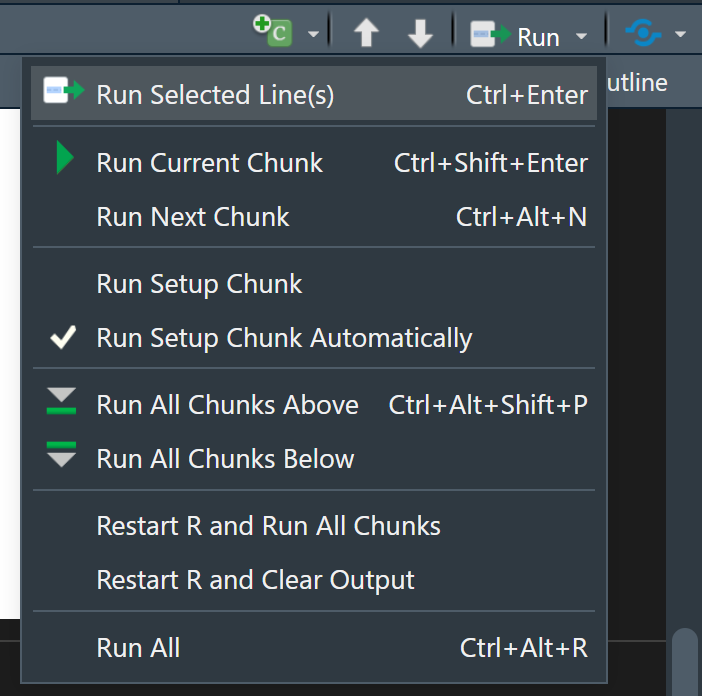
\includegraphics[width=250px]{images/RMarkdown_run_chunk} \end{flushleft}

You can also embed plots, for example:

\includegraphics{Intro_to_R_part2a_markdown_files/figure-latex/unnamed-chunk-3-1.pdf}

Note that the \texttt{echo\ =\ FALSE} parameter was added to the code
chunk to prevent printing of the R code that generated the plot.

You might want to create an object, but not include both the code and
the output in the final \texttt{.html} file. To do this you can use,
include = FALSE. Be aware though, when making reproducible research it's
often not a good idea to completely hide some part of your analysis.

To insert an external figure, you can use the \texttt{include\_graphics}
function in the \texttt{knitr} R package, as shown above in the
screenshot of the run options.

There are several options for inserting tables.

One is the \texttt{kable()} function from the \texttt{knitr} package.
Also checkout the \texttt{gt()} function in the \texttt{gt} package and
the \texttt{pander()} function in the \texttt{pander} package.

\begin{Shaded}
\begin{Highlighting}[]
\FunctionTok{kable}\NormalTok{(pressure)}
\end{Highlighting}
\end{Shaded}

\begin{longtable}[]{@{}rr@{}}
\toprule\noalign{}
temperature & pressure \\
\midrule\noalign{}
\endhead
\bottomrule\noalign{}
\endlastfoot
0 & 0.0002 \\
20 & 0.0012 \\
40 & 0.0060 \\
60 & 0.0300 \\
80 & 0.0900 \\
100 & 0.2700 \\
120 & 0.7500 \\
140 & 1.8500 \\
160 & 4.2000 \\
180 & 8.8000 \\
200 & 17.3000 \\
220 & 32.1000 \\
240 & 57.0000 \\
260 & 96.0000 \\
280 & 157.0000 \\
300 & 247.0000 \\
320 & 376.0000 \\
340 & 558.0000 \\
360 & 806.0000 \\
\end{longtable}

You can manually create small tables using R Markdown syntax. For
example:

\begin{longtable}[]{@{}lcr@{}}
\toprule\noalign{}
Plant & Temp. & Growth \\
\midrule\noalign{}
\endhead
\bottomrule\noalign{}
\endlastfoot
A & 20 & 0.65 \\
B & 20 & 0.95 \\
C & 20 & 0.15 \\
\end{longtable}

There are several other code chunk instructions that you could learn
about (see \textbf{R Markdown Resources} below).

\subsubsection{\texorpdfstring{\textbf{Formatting
text}}{Formatting text}}\label{formatting-text}

Once you knit your document, the output will display text formatted
according to the following simple rules.

\emph{Italic}

Italic

\textbf{Bold}

Bold

This is \texttt{code} in text

This is code in text

\section{Header 1}\label{header-1}

Header 1 (larger font)

\subsection{Header 2}\label{header-2}

Header 2 (smaller font than Header 1)

Note that when a \# symbol is placed inside a code chunk it acts as a
normal R comment, but when placed in text it controls the header size.

\begin{itemize}
\tightlist
\item
  Unordered list item
\end{itemize}

Unordered list item

\begin{enumerate}
\def\labelenumi{\arabic{enumi}.}
\tightlist
\item
  Ordered list item
\end{enumerate}

Ordered list item

\href{https://www.google.com}{Link}

Web link

\(A = \pi \times r^{2}\)

Rendered equation example

The \$ symbols tells R markdown to use LaTeX equation syntax.

\subsubsection{\texorpdfstring{\textbf{Practice}}{Practice}}\label{practice}

To practice this, try writing some formatted text in your \texttt{.Rmd}
document, add some additional code, and produce an \texttt{.html} and
\texttt{.docx} file using the \texttt{Knit} button.

\subsubsection{\texorpdfstring{\textbf{R Markdown
Resources}}{R Markdown Resources}}\label{r-markdown-resources}

Here are some tutorials and other potentially helpful documents. These
same resources are also listed in the ``R Markdown Resources'' page on
Canvas.

Official site\\
- \href{https://rmarkdown.rstudio.com}{Website for R Markdown}

Books (online and free)\\
- \href{https://bookdown.org/yihui/rmarkdown}{R Markdown: The Definitive
Guide}\\
- \href{https://bookdown.org/yihui/rmarkdown-cookbook}{R Markdown
Cookbook}\\
- \href{https://r4ds.had.co.nz/r-markdown.html}{R Markdown \textbar{} R
for Data Science}

Tutorials\\
- \href{https://ourcodingclub.github.io/tutorials/rmarkdown}{Getting
started with R Markdown (Coding Club)}\\
- \href{https://rmarkdown.rstudio.com/authoring_quick_tour.html}{R
Markdown quick tour (RStudio)}\\
-
\href{https://www.dataquest.io/blog/r-markdown-guide-cheatsheet}{Getting
started with R Markdown - Guide and Cheatsheet (Dataquest)}\\
- \href{https://datacarpentry.org/r-socialsci/06-rmarkdown.html}{Getting
started with R Markdown (Data Carpentry)}

\end{document}
